\documentclass[conference]{IEEEtran}
\IEEEoverridecommandlockouts
% The preceding line is only needed to identify funding in the first footnote. If that is unneeded, please comment it out.
\usepackage{cite}
\usepackage{amsmath,amssymb,amsfonts}
\usepackage{algorithmic}
\usepackage{graphicx}
\usepackage{textcomp}
\usepackage{xcolor}
\usepackage{indentfirst}
\usepackage{hyperref}
\usepackage[french]{babel}
\usepackage[T1]{fontenc}
\def\BibTeX{{\rm B\kern-.05em{\sc i\kern-.025em b}\kern-.08em
    T\kern-.1667em\lower.7ex\hbox{E}\kern-.125emX}}
\begin{document}

\title{Communication interplanétaire*\\
{\footnotesize \textsuperscript{*}Comment créer un réseau interplanétaire dans la perspective d'une colonisation de \emph{Mars} ?}
}

\author{\IEEEauthorblockN{Thibault RIVIERE}
\IEEEauthorblockA{\textit{Etudiant en Systèmes Embarqués} \\
\textit{ESEO}\\
Angers, FRANCE \\
thibault.riviere@reseau.eseo.fr}
}

\maketitle

\begin{abstract}
Depuis les premiers pas de l'homme sur la \emph{Lune} en 1969, l'exploration de l'espace a connu de nombreux développements et a suscité de nombreuses questions quant à la possibilité de coloniser d'autres planètes. \emph{Mars}, en particulier, a longtemps été considérée comme un candidat potentiel pour une telle colonisation, en raison de sa proximité avec la Terre et de certaines de ses caractéristiques qui la rendent relativement habitable pour les humains. Cependant, la réalisation d'une telle entreprise nécessitera de revoir profondément les systèmes de communication actuels pour qu'ils soient en mesure de répondre à ces défis.
Dans cet article, nous ferons un état des lieux des technologies actuellement employées. Nous explorerons également les défis techniques et scientifiques à surmonter pour rendre cette vision possible, ainsi que les perspectives d'avenir pour cette technologie.
\newline\textbf{\textit{\hphantom{idt}Mots-clés—}}Communication, périodiquement, exploration, colonisation, revoir profondément les systèmes de communication, amélioration de la communication entre la Terre et \emph{Mars}.
\end{abstract}

\section{Introduction}
Depuis l'avènement du \emph{New Space} et l'intérêt croissant pour l'exploration et la colonisation de l'espace, l'idée d'un réseau interplanétaire capable de relier la Terre à \emph{Mars} et de soutenir la vie humaine sur cette planète a gagné en popularité. Cependant, la création d'un tel réseau comporte de nombreux enjeux et défis, qui doivent être pris en compte pour garantir son efficacité et sa durabilité à long terme.
L'un des principaux défis dans la création d'un réseau interplanétaire est la distance et l'isolement entre les planètes. Les communications entre la Terre et \emph{Mars} peuvent prendre jusqu'à 20 minutes en raison de la distance qui les sépare, ce qui peut rendre la transmission de données et l'interaction en temps réel difficile. De plus, l'environnement hostile de l'espace peut causer des perturbations et des interruptions dans les communications, ce qui peut rendre difficile la \emph{Maintenance} du réseau.
Il s'agit d'un des grands défis technologie du 21e siècle. Pour créer un réseau interplanétaire efficace, il faut développer de nouvelles technologies de communications qui peuvent fonctionner dans l'environnement difficile de l'espace, telles que des antennes et des satellites robustes et fiables pour assurer la durabilité du réseau à long terme.
Enfin, un des autres grands défis est l'importance de la coopération internationale. La création d'un tel réseau nécessite la collaboration de différents pays et organisations, ce qui peut être difficile à réaliser en raison de différences culturelles, politiques et économiques. Il est important que les parties concernées travaillent ensemble de manière transparente et efficace pour atteindre cet objectif.
Ainsi danscet article, nous allons d'abord faire un état des lieux des technologies de communication actuellement utilisées pour les missions spatiales \autoref{sec:DTT}, en mettant en avant les limites de ces technologies. Nous allons ensuite discuter des conjonctions solaires supérieures et de leur impact sur les communications \autoref{sec:HLCS}. Ensuite, nous allons explorer les perspectives d'amélioration de la communication interplanétaire, en mettant en avant les avancées récentes dans le domaine, comme les satellites \emph{Relais} sur les \emph{Points de Lagrange} \autoref{sec:SRPL} ou les technologies de laser \autoref{sec:DTNL}. Enfin, nous conclurons un aperçu des projets en cours et futurs dans le domaine de la communication interplanétaire \autoref{sec:CONC}.

\section{Les dernières tendances technologiques}
\label{sec:DTT}
\subsection{Le \emph{DSN} (\emph{Deep Space Network})}
Actuellement, le réseau Deep Space de la \emph{NASA} est considéré comme le système de télécommunications interplanétaire le plus avancé et le plus performant au monde. Il s'agit d'un réseau international d'antennes radio géantes qui prend en charge les missions d'engins spatiaux interplanétaires et certaines \emph{Orbite} autour de la Terre \cite{b1}. Le \emph{Deep Space Network}, ou \emph{DSN}, est géré par le Jet Propulsion Laboratory de la \emph{NASA}, qui est également responsable de la gestion de nombreuses missions spatiales robotiques de l'agence.
Le \emph{DSN} est composé de trois installations réparties de manière équidistante à environ 120 degrés l'une de l'autre sur l'ensemble du globe. En plus de fournir des communications pour les missions spatiales, le \emph{DSN} permet également des observations radar et de radioastronomie qui contribuent à notre compréhension du système solaire et de l'univers en général.
\newline Ces sites, comme représenté sur la \autoref{fig:locations}, se trouvent à :
\begin{itemize}
\item Goldstone en Californie
\item Madrid en Espagne
\item Canberra en Australie
\end{itemize}

\begin{figure}[htbp]
\centerline{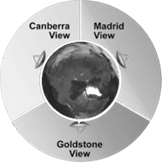
\includegraphics[scale=1.1]{Image1.png}}
\caption{Emplacement des antennes du \emph{DSN} \cite{b2}}
\label{fig:locations}
\end{figure}
L'emplacement stratégique de ces sites permet une communication ininterrompue avec les engins spatiaux grâce à la rotation de notre planète. Lorsqu'un engin spatial se trouve à l'horizon sur un site \emph{DSN}, un autre site peut immédiatement prendre le \emph{Relais} et maintenir les communications. Cette configuration garantit une couverture constante et une transmission de données fluide pour les missions spatiales.
\newline Le réseau \emph{Deep Space Network} (\emph{DSN}) de la \emph{NASA} est un élément clé des \emph{Communications spatiales} lointaines depuis 1963. Il soutient en permanence environ 40 missions et doit faire face à un volume de données en constante augmentation \cite{b3}. En effet, le débit de données des engins spatiaux lointains a été multiplié par plus de 10 depuis les premières missions lunaires dans les années 1960, et cette tendance devrait s'accentuer avec l'envisage de missions humaines vers \emph{Mars}. Pour répondre à ces besoins en constante évolution, le \emph{DSN} est constamment amélioré et mis à niveau. Il a également adopté de nouvelles approches pour gérer les communications dans l'espace lointain \cite{b4}, comme la possibilité de recevoir plusieurs signaux d'une seule antenne grâce à un protocole de traitement numérique.
En outre, les communications optiques, qui utilisent des lasers pour permettre une communication à haut débit, sont un autre outil qui pourrait aider à répondre à la demande croissante en volume de données. La \emph{NASA} a prévu plusieurs missions pour démontrer cette technologie dans les années à venir.

\subsection{Le \emph{DTN} (\emph{Delay Tolerant Network})}
\subsubsection{\textbf{\textit{Principes théoriques}}}
L'architecture de réseau tolérante aux délais et aux interruptions, ou \emph{DTN} (\emph{Delay Tolerant Network}), a été développée dans le domaine de l'aérospatiale.  Cette architecture est un modèle de surcouche réseau tolérante aux délais et aux interruptions \cite{b5}. Elle est représentée par un réseau de nœuds interconnectés, à l’aide d’une couche dite \emph{Bundle}. Cette couche se place entre la couche applicative et la couche transport. Elle permet de mettre en œuvre le réseau via deux mécanismes, qui sont le store- and-forward et la couche de convergence.
\newline En effet, le premier mécanisme de \emph{Store-and-forward} \autoref{fig:store-and-forward} est un mécanisme de stockage longue durée des données au niveau des nœuds intermédiaires. Ces nœuds stockent le message et vérifient son intégrité avant de le transmettre au nœud suivant, et ce jusqu’à ce que le message arrive à destination \cite{b6}. Ce transfert est ce qu’on appelle un custody transfert \cite{b7}. 

\begin{figure}[htbp]
\centerline{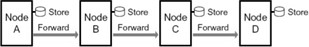
\includegraphics[scale=1.1]{Image2.jpg}}
\caption{Mécanisme de \emph{Store-and-forward} \cite{b7}}
\label{fig:store-and-forward}
\end{figure}
Contrairement au protocole \emph{TCP/IP} classique dont la transmission des données est effectuée par la couche applicative, le stockage persistant des bundles permet au nœud \emph{DTN} de déléguer cette charge au nœud voisin en même temps que le \emph{Bundle} effectif.
Par ce premier mécanisme, il est possible de communiquer dans des conditions difficiles et ce, pour plusieurs raisons. Premièrement, les nœuds intermédiaires sont capables de retransmettre directement l’information. Ceci permet d’éviter des pertes de données très coûteuses lors de la communication.
D’autre part, la communication \emph{Store-and-forward} permet grâce au système à étapes, de s’assurer que la transmission de données d’un \emph{Bundle} à un nœud voisin est effectuée avec succès. Cette avancée par étape assure un acheminement de l’information dans les environnements même les plus contraints ou extrêmes. Par exemple, pour des réseaux spatiaux caractérisés par de grandes pertes, la gestion de la transmission nœud par nœud (donc étape par étape) permet de gagner en efficacité et d’éviter au maximum les pertes de données.
Le second mécanisme permettant de mettre en œuvre un réseau \emph{DTN}, est la couche de
convergence. Cette couche fait le lien entre la couche \emph{Bundle} et les couches inférieures
(Transport, etc.). Par ailleurs, du fait que le réseau \emph{DTN} soit un réseau de surcouche sans réelles contraintes, la couche de convergence induit la possibilité d’interconnexion de régions hétérogènes.
En effet, grâce à la couche de convergence, il est possible de communiquer via des protocoles différents en passant par le réseau \emph{DTN} et ce, sans devoir utiliser de passerelles. La couche agit à ce moment précis telle une couche réseau, de la même manière que le protocole IP permet d’interconnecter des machines. Enfin, il semble important de noter que la couche de convergence est confondue avec la couche \emph{Bundle} dans son fonctionnement.
\subsubsection{\textbf{\textit{Méthodes couramment utilisées}}}
Actuellement, le réseau \emph{DTN} prend place dans la conquête spatiale et s’inscrit dans les objectifs du Comité consultatif sur les systèmes de données spatiales (\emph{CCSDS}). En effet, l’un des objectifs de ce comité est la \emph{Standardisation} de cette architecture. C’est pourquoi, depuis plusieurs années, ce réseau se démocratise dans le domaine du \emph{New Space} : de plus en plus d’entreprises s’y intéressent et l’expérimentent.
La première expérimentation connue d’un \emph{DTN} spatial a été initiée par le Laboratoire de recherche sur la propulsion par réaction (ou Jet Propulsion Laboratory) de la \emph{NASA}, en 2008. Le réseau \emph{DTN} a été installé et testé sur la sonde Deep Impact du vaisseau \emph{EPOXI}. Grâce au réseau, les informations ont pu être stockées lors de l’interruption des communications et transmises à destination à l’aide de \emph{Relais} une fois la communication rétablie.
Cette expérience du nom de \emph{Deep Impact Network Experiment} (\emph{DINET}) a permis la transmission de 300 images des nœuds du laboratoire de la \emph{NASA} en Californie au vaisseau \emph{EPOXI}, à 32 millions de kilomètres de la Terre.
De nos jours, la mise en place du réseau \emph{DTN} dans le domaine de l’aérospatiale s’est développée. En effet, \emph{DTN} a également eu l’occasion d’être expérimenté sur l’\emph{ISS} et à travers une nouvelle technologie de \emph{Faisceau laser} pulsé provenant de la \emph{Lune} \cite{b8}.


\subsection{Le module \emph{HLCS} (\emph{Halo Lunar Communication System})}
\label{sec:HLCS}
Dans le cadre du projet international \emph{Artémis}, l'Agence Spatiale Européenne (\emph{ESA}) a signé un contrat avec Thales Alenia Space pour développer un nouveau module de communication et de ravitaillement, appelé ESPRIT (European System Providing Refueling, Infrastructure and Télécommunications), autour de la \emph{Lune}. Ce module sera lancé en 2026 et sera composé du module \emph{HLCS} (\emph{Halo Lunar Communication System}), qui assurera les communications entre la Terre, la station Gateway et la \emph{Lune} \cite{b9}.
Bien que l'objectif principal du module ESPRIT soit principalement de garantir la communication entre la Terre et la \emph{Lune}, il est admis qu'il pourrait également servir de \emph{Relais} pour de futures missions vers \emph{Mars}, qui décolleraient très probablement de la future station lunaire.
Cependant, malgré son équipement de dernière génération et comme tout équipement de communication terrestre ou en \emph{Orbite}, il souffre d'une grande faiblesse qui rend inopérant tout moyen de communication pendant de longue période. Les conjonctions solaires supérieures (\emph{SSC}) sont des périodes où le Soleil se trouve entre la Terre et \emph{Mars}, ce qui bloque les communications entre les deux planètes \autoref{fig:SSC}. Pendant ces périodes, les communications par ondes radio sont perturbées en raison de l'interférence causée par la radiation solaire. Cela peut entraîner des pannes de communication pouvant aller jusqu'à 78 jours, selon le système de communication utilisé. Les systèmes à bande passante plus élevée sont plus vulnérables à ces perturbations.

\begin{figure}[htbp]
\centerline{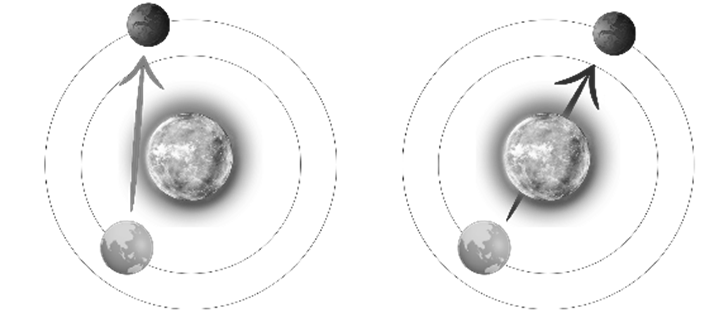
\includegraphics[scale=1.18]{Image3.png}}
\caption{\emph{conjonction solaire supérieure} (\emph{SSC}) \cite{b9}}
\label{fig:SSC}
\end{figure}

Il est important de noter que les conjonctions solaires supérieures ne bloquent pas seulement les communications entre la Terre et \emph{Mars}, mais aussi entre la Terre et tout autre corps céleste situé derrière le Soleil. Cela signifie que les communications avec des vaisseaux spatiaux ou des sondes situées au-delà de \emph{Mars} peuvent également être perturbées pendant ces périodes \cite{b10}.


\section{Perspectives d'amélioration}
\subsection{Satellites \emph{Relais} sur les \emph{Points de Lagrange}}
\label{sec:SRPL}
Un point de Lagrange est un point de l'espace où la gravitation de deux corps massifs, tels que la Terre et la \emph{Lune}, s'annule. Cela permet à un objet placé à cet endroit de rester en \emph{Orbite} stable, sans avoir besoin de propulseur pour maintenir sa position.
Il existe cinq \emph{Points de Lagrange} dans le système Terre-\emph{Lune}, connus sous les noms de L1, L2, L3, L4 et L5. Chacun d'entre eux se trouve à une distance spécifique de la Terre ou de la \emph{Lune} et possède des caractéristiques uniques en termes de conditions environnementales et de possibilités d'observation.
Les \emph{Points de Lagrange} sont souvent utilisés comme bases de lancement pour les missions spatiales, car ils permettent de minimiser l'utilisation de carburant pour atteindre d'autres destinations dans l'espace. Ils sont également utilisés pour observer l'environnement spatial et l'univers lointain, car ils offrent une vue dégagée sur le ciel \autoref{fig:Lagrange} \cite{b10}.

\begin{figure}[htbp]
\centerline{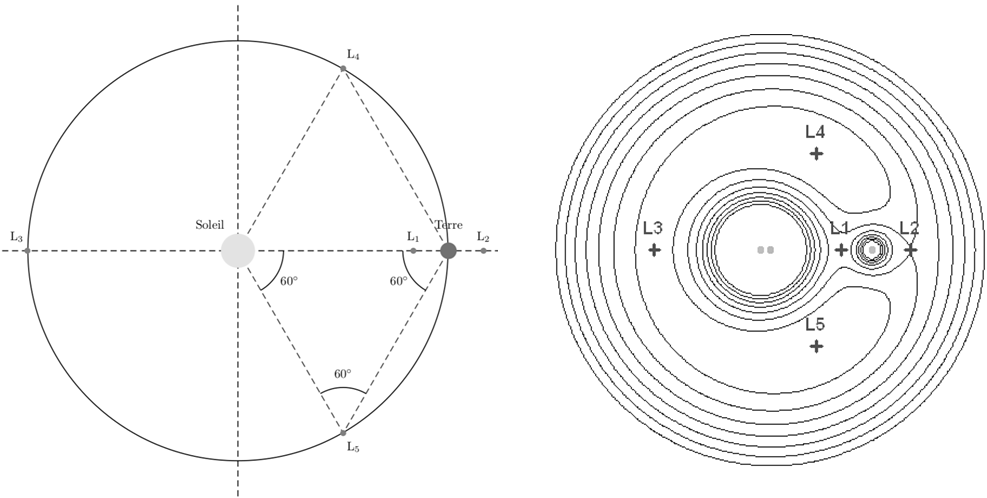
\includegraphics[scale=1.26]{Image4.png}}
\caption{\emph{Points de Lagrange} du système Soleil/Terre \cite{b11}}
\label{fig:Lagrange}
\end{figure}

Tout comme le système Terre-\emph{Lune}, chaque planète du système solaire possède un ensemble de cinq \emph{Points de Lagrange} qui lui sont associés et qui sont en relation avec le Soleil. Ces points, appelés L4 et L5, sont visibles depuis n'importe quelle autre planète du système solaire, indépendamment de la position du Soleil par rapport aux deux. Ils ont donc une grande valeur en tant que points de \emph{Relais} pour les communications, car ils permettent d'éviter les pannes de communication dues aux conjonctions solaires. Il existe quatre ensembles de \emph{Points de Lagrange} solaires qui pourraient être utilisés à cet effet: 
\begin{itemize}
\item Mars-Soleil - L4 et L5
\item Terre-Soleil - L4 et L5
\item Vénus-Soleil - L4 et L5
\item Mercure-Soleil - L4 et L5
\end{itemize}
Pour déterminer le système de satellites \emph{Relais} le plus adapté à nos futurs besoins, il est important de prendre en compte les progrès technologiques récents (ex: James Webb Space Telescope (\emph{JWST}))  ainsi que les satellites de télécommunications existants. Ce système aura des implications non seulement pour les architectures de mission humaine sur \emph{Mars}, mais également pour les architectures d'exploration \cite{b10}.
Les missions Lunaire du projet \emph{Artémis} sont aussi étudiées dans le but de préparer les futures missions humaines vers \emph{Mars}, car il est crucial de s'assurer que les systèmes de satellites \emph{Relais} fonctionnent de manière optimale avant de les mettre en \emph{Orbite} autour des \emph{Points de Lagrange}. En effet, une fois en place, il sera impossible de procéder à des \emph{Maintenance} ou à des réparations sur ces satellites en raison de la distance colossale qui les sépare de la Terre. C'est pourquoi il est essentiel de tester ces systèmes de manière approfondie afin de garantir leur \emph{Fiabilité} à long terme pour les missions futures vers \emph{Mars} \cite{b12}.

\subsection{Le \emph{DTN} (\emph{Delay Tolerant Network}) à l'échelle du système solaire}
\label{sec:DTNL}
Le réseau \emph{Delay Tolerant Network} admet de nombreux avantages, dont notamment le stockage longue durée des paquets. En effet, la structure de ce réseau permet lorsqu’une communication ne peut être établie, de garder les paquets de données dans un nœud jusqu’à ce que la liaison soit rétablie. La perte de données est donc moindre comparée à un protocole \emph{TCP/IP} classique, dans lequel les paquets de données sont rejetés lors que le destinataire est introuvable ou injoignable.
Cette méthode de stockage et transfert des données est sécurisante pour l’émetteur, qui n’émet aucun doute sur le fait que le paquet de données arrivera un jour à destination. Les données ne sont pas perdues lorsqu’il n’existe aucun chemin immédiat vers la destination.
Par ailleurs, grâce au \emph{DTN} la communication est possible sur des milliers de kilomètres. Il permet notamment grâce au procédé de multi routage, de transmettre efficacement des données dans des situations qui impliquent des déconnexions, des délais (lors de missions spatiales) ou encore, des inadéquations de débits \cite{b13}. 
Enfin, c’est un réseau normé. Cela sous-entend que la réutilisation de celui-ci pour des missions ou applications futures est favorisée. De plus, \emph{DTN} possède des qualités d’interopérabilité, puisqu’il est capable de fonctionner avec des systèmes existants ou futurs et ce, sans restriction d’accès ou de mise en œuvre \cite{b14}\cite{b15}. 
Malgré tous les avantages cités précédemment, le réseau \emph{DTN} admet quelques limites. Parmi ces limites, il convient notamment de citer le délai de transmission. En effet, celui-ci s’avère plus ou moins long en fonction de la probabilité de rencontre des nœuds. Comme précédemment expliqué, dans le cas où une liaison ne peut être établie à l’instant t, le paquet de données est stocké dans le tampon d’un nœud et ce, jusqu’à ce que le paquet soit transmissible (soit lorsque la connexion est établie vers un nœud voisin) \cite{b16}.
Ce délai de mise en file d’attente peut être extrêmement long dans certains cas, puisqu’il relate de l’environnement extérieur entre l’émetteur et le récepteur. Par exemple, si la transmission du paquet de la Terre vers \emph{Mars} est bloquée par le Soleil, les informations seront stockées et relayées une fois la communication possible.
Enfin, comme toute technologie \emph{DTN} est limité en termes de ressources. En effet, la capacité de stockage dans la mémoire tampon d’un nœud est limitée. Tout comme la capacité de traitement des informations, la batterie d’un nœud ou encore sa disponibilité.
La \emph{NASA} va prochainement mener une expérience de communication de ce type pour juin 2023. L'agence américaine embarquera cette technologie à bord d'un satellite expérimental de l'US Air Force, qui devra relayer des données entre les missions spatiales et la Terre. Ce premier test devrait notamment permettre de transmettre sur Terre les données scientifiques recueillies par l'Illuma-T, terminal optique installé sur l'\emph{ISS}. 

\section{Conclusion}
\label{sec:CONC}
Les projets spatiaux envisagés et initiés concernent des zones beaucoup plus éloignées que l'\emph{Orbite} terrestre utilisée par la Station Spatiale Internationale (\emph{ISS}). Ces missions spatiales génèrent et collectent de grandes quantités de données, ce qui augmente la nécessité d'améliorer les capacités de communication à l’échelle interplanétaire.
L'une des options explorées par les agences spatiales est le réseau \emph{DTN} par laser, qui pourrait augmenter de dix fois le débit de données tout en réduisant la taille, la consommation électrique et le poids des équipements de communication. 
De plus, le \emph{DTN} pourrait être couplé à un système de satellites \emph{Relais} placés sur les \emph{Points de Lagrange} pour assurer une portée suffisante pour nos besoins. Cependant, aucune agence n'a encore lancé d'appel d'offres pour un système équivalent, ce qui laisse penser que ce type de système ne sera pas opérationnel avant plusieurs décennies.
Il est important de noter que l'utilisation de la technologie \emph{DTN} par laser n'est pas la seule piste explorée pour améliorer la communication interplanétaire. D'autres agences spatiales et entreprises privées travaillent également sur des moyens de communication plus efficaces et fiables pour les missions spatiales lointaines. Par exemple, SpaceX a annoncé son projet de déploiement de sa constellation de satellites Starlink autour de \emph{Mars} pour soutenir les futurs voyageurs spatiaux. En outre, l'Agence spatiale européenne (\emph{ESA}) travaille sur le développement du module de communication et de ravitaillement ESPRIT (European System Providing Refueling, Infrastructure and Télécommunications) dans le cadre du projet international \emph{Artémis}. Ce module sera lancé en 2026 et sera composé du module \emph{HLCS} (\emph{Halo Lunar Communication System}) qui assurera les communications entre la Terre, la station Gateway et la Lune. Il est également admis que le module ESPRIT pourrait être utilisé comme \emph{Relais} pour de futures missions vers \emph{Mars}.
Il est évident que l'amélioration de la communication interplanétaire est cruciale pour assurer le succès des missions spatiales futures et pour maintenir une communication efficace entre les différentes parties impliquées dans ces missions \cite{b17}.

\clearpage

\appendix
Dictionnaire de domaine :
\begin{itemize}
\item NASA : National Aeronautics and Space Administration, plus connue sous son acronyme NASA, est l'agence fédérale responsable de la majeure partie du programme spatial civil des États-Unis.
\item ESA : Agence spatiale européenne, le plus souvent désignée par son sigle anglais ESA, est une agence spatiale intergouvernementale coordonnant les projets spatiaux menés en commun par 22 pays européens.
\item CCSDS : Comitée consultatif sur les systèmes de données spatiales, organisme international qui promeut la \emph{Standardisation} et la coopération dans les \emph{Communications spatiales} et les systèmes de données pour les missions spatiales.
\item Communications spatiales: la transmission de données et de commandes entre les engins spatiaux et les centres de contrôle sur Terre.
\item Deep Space Network (DSN) : système de communications de la \emph{NASA} qui soutient les missions spatiales lointaines depuis 1963.
\item DTN (Delay Tolerant Network) : architecture de réseau tolérant aux délais et aux interruptions, utilisée pour les \emph{Communications spatiales} lointaines.
\item Store-and-forward : mécanisme de stockage à long terme des données dans les nœuds intermédiaires d'un réseau \emph{DTN}.
\item DINET : Deep Impact Network Experiment, une expérience de transmission de données menée par la \emph{NASA} en utilisant le réseau \emph{DTN} sur la sonde Deep Impact.
\item TCP/IP : protocole de communication utilisé pour transmettre des données sur un réseau informatique, comprenant une couche de transport (TCP) et une couche de réseau (IP). Il est utilisé pour les communications Internet et est considéré comme le protocole de communication standard pour les réseaux informatiques.
\item Bundle : couche de communication dans un réseau \emph{DTN} qui permet la mise en œuvre du \emph{Store-and-forward} et de la couche de convergence.
\item SSC : conjonction solaire supérieure, période durant laquelle le Soleil se trouve entre la Terre et une autre planète, entraînant une interruption de communication.
\item Points de Lagrange : points de l'espace où les forces gravitationnelles de deux corps en \emph{Orbite} se compensent, pouvant être utilisés comme points de \emph{Relais} pour les \emph{Communications spatiales}.
\item ISS : Station spatiale internationale, plateforme d'expérimentation en microgravité.
\item Artémis : projet international de l'ESA visant à établir une présence humaine durable sur la \emph{Lune}.
\item ESPRIT (European System Providing Refueling, Infrastructure and Télécommunications) : module de communication et de ravitaillement autour de la \emph{Lune} dans le cadre du projet \emph{Artémis}.
\item HLCS (Halo Lunar Communication System) : composante du module ESPRIT qui assurera les communications entre la Terre, la station Gateway et la \emph{Lune}.
\item James Webb Space Telescope (JWST) : télescope spatial à haute résolution qui permettra d'étudier les premières étoiles et galaxies de l'Univers.
\item EPOXI : vaisseau spatial lancé en 2005 pour étudier la comète Tempel 1 et la planète naine Cérès.
\item Système solaire : ensemble des corps célestes qui gravitent autour du Soleil, comprenant les planètes, les lunes, les astéroïdes et les comètes.
\item Mission humaine : projet visant à envoyer des êtres humains dans l'espace pour explorer et étudier les corps célestes.
\item Mars : planète rouge la plus proche de la Terre, objet de nombreuses missions d'exploration spatiale en raison de sa proximité et de sa potentielle habitabilité.
\item Lune : satellite naturel de la Terre, cible de nombreuses missions d'exploration spatiale en raison de sa proximité et de son rôle dans les \emph{Communications spatiales}.
\item Exploration spatiale : processus d'enquête et de découverte de l'espace en utilisant des moyens technologiques.
\item Missions spatiales : projets visant à envoyer des engins spatiaux pour explorer et étudier les corps célestes dans l'espace.
\item Standardisation : processus de normalisation pour assurer la compatibilité et l'interopérabilité des systèmes et technologies.
\item New Space : secteur émergent de l'industrie spatiale qui comprend les entreprises non gouvernementales et les projets commerciaux dans l'espace.
\item Fiabilité : capacité d'un système à fonctionner de manière fiable et fiable dans des conditions données.
\item Maintenance : processus de réparation et d'entretien d'un équipement ou d'un système pour maintenir son bon fonctionnement et prolonger sa durée de vie.
\item Orbite : parcours régulier et répétitif d'un corps céleste autour d'un autre corps céleste sous l'effet de la gravité.
\item Vaisseau spatial : engin conçu pour voyager dans l'espace, transportant des êtres vivants ou des instruments scientifiques.
\item Sonde spatiale : engin spatial automatisé destiné à étudier un corps céleste ou un phénomène spatial.
\item Relais : dispositif qui reçoit et transmet des signaux ou des données à travers un réseau.
\item Faisceau laser : système utilisant des rayons laser pour transmettre des données à grande distance dans l'espace.
\end{itemize}

\clearpage

\begin{thebibliography}{00}
\bibitem{b1} MONAGHAN, Heather, NASA Jet Propulsion Laboratory, What is the Deep Space Network, Mar. 2020.
\bibitem{b2} Lindsay Johnson, My Space, Ever wondered How NASA is still in contact with the Voyagers?, Jun. 2021.
\bibitem{b3} NASA, Jet Propulsion Laboratory, California Institute of Technology, Deep Space Network Now, Jan. 2023.
\bibitem{b4} O'NEILL, Ian J., FAUCONNET, Laurance, GREICIUS, Tony, NASA Jet Propulsion Laboratory, NASA’s Deep Space Network Looks to the Future, Sep. 2021.
\bibitem{b5} GREFF, Florian. Vers l’Internet interplanétaire : mise en œuvre d’un réseau DTN dans un contexte de simulation d’une liaison spatiale. 2014.
\bibitem{b6} WARTHMAN, Forrest, et al. Delay-and disruption-tolerant networks (DTNs). A Tutorial. V.. 0, Interplanetary Internet Special Interest Group, 2012, p. 5-9.
\bibitem{b7} YU, Yang et CHEN, Xiaomin. Performance evaluation of custody transfer in Mars-to-Earth DTN communications. In : 2013 IEEE International Conference on Signal Processing, Communication and Computing (ICSPCC 2013). IEEE, 2013. p. 1-5.
\bibitem{b8} TZINIS, Irene - Disruption Tolerant Networking (DTN) Tested on Spacecraft, Oct. 2008.
\bibitem{b9} Dynetics, Thales Alenia Space/Briot, Esa, Nasa. Thales Alenia Space : au cœur des plus grand
défis industriels. 2021.
\bibitem{b10} CORNISH, Neil J., NASA Solar System Exploration, WMAP Science Team, What is a Lagrange Point, Mar. 2018
\bibitem{b11} Esa, The five Lagrange points, May 2021.
\bibitem{b12} CoconutScienceLab, How Will the Martian Rovers Deal With Solar Conjunction, Mar. 2013.
\bibitem{b13} MONAGHAN, Heather, NASA, Delay/Disruption Tolerant Networking, Sep. 2020.
\bibitem{b14} AIDI, Laili et CHANGSU, Jung. Delay Tolerant Network. 2012.
\bibitem{b15} HOOKE, A. J., BURLEIGH, S., CERF, V., et al. The interplanetary internet: a communications infrastructure for Mars exploration. 2002.
\bibitem{b16} CHOUDHARY, Lalitesh Kumar, AHIRWAR, Manish Kumar, et CHAURASIYA, Uday. Practical Routing Strategy in Delay-Tolerant Networks: A Survey. International Journal of Computer Science and Information Security, 2013, vol. 11, no 7, p. 25.
\bibitem{b17} Orange, Astro\_TJ. Laser, protocole et matériel dédiés : l’avenir des télécoms spatiales, 2021.
\end{thebibliography}
\end{document}
